\documentclass[11pt,a4paper]{article}

% Version 1.0

\usepackage{amsmath,amssymb,amsfonts}
\usepackage{graphicx}
\usepackage{physics}
\usepackage{hyperref}
\usepackage{geometry}
\geometry{margin=3cm}

\title{Why Is the Sky Blue?\\
A Geometric Derivation of Rayleigh Scattering from Maxwell Theory}

\author{Gustaf Ullman}

\date{\today}

\begin{document}

\maketitle

\begin{abstract}
The usual answer to the question why the sky is blue is that shorter
wavelengths of sunlight are scattered more efficiently by the atmosphere
than longer wavelengths. This answer is correct, but incomplete: it names
the relevant effect without displaying the physical chain that produces it.
This paper gives a conceptually explicit derivation of Rayleigh scattering
from Maxwell theory, with particular attention to the geometrical structure
of the electromagnetic field.

The aim is not pedagogical in the sense of simplification. It is structural:
to make visible how a familiar phenomenon follows from the geometrical and
dynamical structure of Maxwell theory. The intended reader is assumed to have
some background in classical electrodynamics and relativity. The guiding idea
is conceptual seeing: the Rayleigh law is not treated as a formula to be
remembered, but as a consequence of the structure through which the phenomenon
becomes physically intelligible.

The central chain is that an incident electromagnetic field polarizes a small
molecule, the induced dipole radiates according to Maxwell's equations, the
far-zone radiation field is proportional to the second time derivative of the
dipole moment, and the observed intensity is obtained from the electromagnetic
stress-energy structure, which is quadratic in the field. For harmonic
radiation this gives a scattered field amplitude proportional to \(\omega^2\),
and hence an intensity proportional to \(\omega^4\), or equivalently to
\(\lambda^{-4}\). A brief quantum interpretation is also included: Rayleigh
scattering may be represented as a second-order process involving virtual
molecular excitations, but it should not be confused with real absorption
followed by de-excitation.

The derivation is then recast in spacetime algebra, where the electromagnetic
field is represented as a bivector \(F\), the electric and magnetic fields are
observer-dependent projections of \(F\), and the stress-energy tensor becomes
the vector-valued linear map
\[
T_F(a)= -\frac{\varepsilon_0}{2}FaF.
\]
In this formulation Rayleigh scattering appears as a geometric process: an
incident bivector field is projected in the molecular rest frame, induces a
transverse oscillating dipole, generates an outgoing radiation bivector, and
yields an observed energy flux through the stress-energy map.
\end{abstract}

\section{Introduction}

The blue colour of the sky is usually explained by saying that blue light is
scattered more strongly than red light in the Earth's atmosphere. This is
true, but it is not yet a full physical explanation. It gives the name and
qualitative direction of the effect, but it does not yet explain why the
scattering strength should scale as the inverse fourth power of wavelength.

The relevant mechanism is Rayleigh scattering. It applies when the scattering
object is much smaller than the wavelength of the incident radiation. Air
molecules have a typical size of order \(10^{-10}\,\mathrm{m}\), while visible
light has wavelengths of order \(4\cdot 10^{-7}\) to
\(7\cdot 10^{-7}\,\mathrm{m}\). Thus, for visible light in the atmosphere, the
molecular scatterers are very small compared with the wavelength.

The purpose of this paper is not to give an elementary or popular account of
the blue sky. The aim is instead structural clarification. By this I mean an
explanation that does not merely attach a formula to a phenomenon, but makes
visible the chain of physical and geometrical dependencies through which the
phenomenon becomes intelligible. The intended reader is assumed to have some
familiarity with classical electromagnetism, including Maxwell's equations,
radiation from accelerated charges, and the Poynting vector.

In this respect the paper is also a small exercise in conceptual seeing. In a
sense close to Hanson's account of theory-laden observation, a physical
phenomenon becomes intelligible when it is seen under the right theoretical
structure. The blue sky is not fully explained by attaching the phrase
``short wavelengths scatter more'' to it. It becomes intelligible when the
Rayleigh law is seen as the joint consequence of induced molecular
polarization, dipole radiation, and the quadratic stress-energy structure of
the electromagnetic field.

The role of spacetime algebra is not to make the mathematics superficially
easier. Rather, it displays more clearly the geometric unity of the
electromagnetic field, observer-dependent field decompositions, and
stress-energy flow. In STA the electromagnetic field is not fundamentally a
pair \((\mathbf{E},\mathbf{B})\), but a single spacetime bivector \(F\).
Electric and magnetic fields arise only after choosing a timelike direction
\(u\), that is, after specifying an observer or physical rest frame.

This also changes how the frequency dependence should be read. The frequency
that enters the molecular response is not an absolute property of the wave
alone. It is the frequency measured in the rest frame of the scatterer, given
geometrically by the projection of the incident null wave vector \(k\) onto the
molecular four-velocity \(u\):
\[
\omega = k\cdot u,
\]
up to conventional factors of \(c\). Thus the \(\omega^4\) dependence in the
Rayleigh law is already tied to a physically realized observer projection.

In the Rayleigh regime the incident electromagnetic field is nearly uniform
across each molecule. The field polarizes the molecule, displacing its electron
cloud slightly relative to its nuclei. The molecule becomes a small induced
electric dipole. Since the incident field oscillates, the induced dipole also
oscillates. An oscillating dipole radiates. The scattered light is the
radiation field of this driven dipole.

The familiar Rayleigh law is

\begin{equation}
I_{\mathrm{sc}} \propto \frac{1}{\lambda^4}.
\end{equation}

The derivation has two essential steps.

First, the far radiation field of an oscillating dipole is proportional to the
second time derivative of the dipole moment. For harmonic radiation of angular
frequency \(\omega\), this gives a factor \(\omega^2\) in the field amplitude.

Second, intensity is not proportional to field amplitude but to energy flux.
Electromagnetic energy flux is quadratic in the field. In conventional vector
notation this is expressed by the Poynting vector,

\begin{equation}
\mathbf{S} = \frac{1}{\mu_0}\mathbf{E}\times\mathbf{B}.
\end{equation}

In relativistic form it is part of the electromagnetic stress-energy tensor.
Thus an \(\omega^2\) dependence in the radiation field amplitude becomes an
\(\omega^4\) dependence in intensity.

The blue sky is therefore not merely an elementary optical phenomenon. It is a
macroscopic trace of the geometry and dynamics of Maxwell theory.

\section{The Rayleigh Regime}

Rayleigh scattering applies when the characteristic size \(a\) of the
scatterer is much smaller than the wavelength \(\lambda\) of the incident
radiation:

\begin{equation}
a \ll \lambda.
\end{equation}

In this limit the electric field of the incident wave is approximately
constant over the molecule. The molecule need not be treated as an extended
object with appreciable phase differences across it. To leading order it may
be treated as a pointlike polarizable system.

For an isotropic molecule, the induced electric dipole moment is proportional
to the local electric field:

\begin{equation}
\mathbf{p}(t) = \alpha \mathbf{E}(t),
\end{equation}

where \(\alpha\) is the molecular polarizability. If the incident wave is
monochromatic,

\begin{equation}
\mathbf{E}(t) = \mathbf{E}_0 \cos(\omega t),
\end{equation}

then

\begin{equation}
\mathbf{p}(t) = \mathbf{p}_0 \cos(\omega t),
\qquad
\mathbf{p}_0 = \alpha \mathbf{E}_0.
\end{equation}

This is the elementary physical model behind Rayleigh scattering: a small
polarizable molecule becomes a driven oscillating electric dipole. The
derivation does not require the molecule to absorb and re-emit light as a
sequence of separate events. In the classical description, the incident field
drives a bound charge distribution, and the driven charge distribution
radiates.

There is, however, a useful quantum qualification. Rayleigh scattering should
not be understood as ordinary absorption followed by emission through a real
excited molecular state. Far from resonance, the molecule responds
elastically: it returns to its initial state and the outgoing photon has the
same frequency as the incoming photon, apart from negligible recoil effects.
In quantum language, the process may be described as a second-order process in
which the incident photon couples to virtual molecular excitations before an
outgoing photon is emitted. The virtual intermediate states contribute to the
frequency-dependent polarizability of the molecule, but they are not real
long-lived excitations. Thus the classical induced-dipole picture and the
quantum virtual-transition picture are not competing explanations. They are
different descriptions of the same off-resonant elastic response.

\section{A Bound Electron Model}

One can see the origin of the induced dipole more explicitly by modelling a
bound electron as a driven oscillator. Let \(x\) be the displacement of an
electron of charge \(-e\) and mass \(m\) from its equilibrium position. In a
simple classical model,

\begin{equation}
m\ddot{x} + m\gamma \dot{x} + m\omega_0^2 x
=
-e E_0 \cos(\omega t),
\end{equation}

where \(\omega_0\) is the characteristic binding frequency and \(\gamma\) is a
damping coefficient.

For frequencies far below resonance, \(\omega \ll \omega_0\), and ignoring
damping for simplicity, the displacement is approximately

\begin{equation}
x(t) \approx -\frac{e}{m\omega_0^2}E_0 \cos(\omega t).
\end{equation}

The dipole moment is \(p=-ex\), so

\begin{equation}
p(t) \approx \frac{e^2}{m\omega_0^2}E_0\cos(\omega t).
\end{equation}

Thus the polarizability is, in this simple model,

\begin{equation}
\alpha \approx \frac{e^2}{m\omega_0^2}.
\end{equation}

Real molecular polarizabilities are more complicated, and for a full treatment
one must take into account molecular structure, anisotropy, resonances, and
quantum effects. None of these complications changes the basic point needed
for the Rayleigh law: far from resonance and for scatterers much smaller than
the wavelength, the leading response is dipolar and linear in the incident
field.

In quantum theory, the same polarizability can be understood as encoding the
coupling of the molecular ground state to excited states through the electric
dipole operator. Schematically,

\begin{equation}
\alpha(\omega)
\sim
\sum_n
\left(
\frac{|\langle n|\mathbf{d}|0\rangle|^2}{E_n-E_0-\hbar\omega}
+
\frac{|\langle n|\mathbf{d}|0\rangle|^2}{E_n-E_0+\hbar\omega}
\right),
\end{equation}

with appropriate tensor indices and constants suppressed. This expression is
not needed for the classical derivation below, but it clarifies the physical
meaning of the off-resonant response. The molecule need not be truly excited
in order to be polarizable. The possible excited states enter virtually,
through the response function \(\alpha(\omega)\).

\section{Radiation from an Oscillating Dipole}

Maxwell's equations imply that accelerated charges radiate. In the far zone,
the electric field radiated by a localized time-dependent electric dipole
\(\mathbf{p}(t)\) is

\begin{equation}
\mathbf{E}_{\mathrm{rad}}(\mathbf{r},t)
=
\frac{1}{4\pi\varepsilon_0 c^2 r}
\left[
\hat{\mathbf{n}}
\times
\left(
\hat{\mathbf{n}}
\times
\ddot{\mathbf{p}}(t_r)
\right)
\right],
\end{equation}

where

\begin{equation}
t_r = t - \frac{r}{c}
\end{equation}

is the retarded time, and \(\hat{\mathbf{n}}\) is the unit vector from the
dipole to the observer.

The double cross product projects the dipole acceleration onto the plane
transverse to the observation direction. This expresses an important physical
fact: radiation fields are transverse.

For a harmonic dipole,

\begin{equation}
\mathbf{p}(t) = \mathbf{p}_0 \cos(\omega t),
\end{equation}

we have

\begin{equation}
\ddot{\mathbf{p}}(t) = -\omega^2 \mathbf{p}_0 \cos(\omega t).
\end{equation}

Therefore the amplitude of the radiated electric field is proportional to

\begin{equation}
E_{\mathrm{rad}} \propto \omega^2 p_0.
\end{equation}

Since \(p_0=\alpha E_0\), the scattered field amplitude is proportional to

\begin{equation}
E_{\mathrm{sc}} \propto \omega^2 \alpha E_0.
\end{equation}

This is the first essential step in the Rayleigh law. The fourth power has
not yet appeared. At this stage we have only obtained a second power in
frequency at the level of field amplitude.

\section{Energy Flux and the Poynting Vector}

The observed brightness of light is not proportional to the electric field
amplitude itself. It is proportional to electromagnetic energy flux.

In conventional vector notation the electromagnetic energy flux is given by
the Poynting vector,

\begin{equation}
\mathbf{S}
=
\frac{1}{\mu_0}\mathbf{E}\times\mathbf{B}.
\end{equation}

This expression is not an arbitrary definition of optical intensity. It follows
from Maxwell's equations when they are written as a local energy conservation
law. The electromagnetic energy density is

\begin{equation}
u_{\mathrm{em}}
=
\frac{1}{2}\varepsilon_0 E^2
+
\frac{1}{2\mu_0}B^2.
\end{equation}

It is worth emphasizing what this quadratic dependence means physically. The
electric field \(\mathbf{E}\) is not itself an energy. It has the dimension of
force per unit charge. The energy density arises only when the field strength
is combined with the electromagnetic constants. In SI units,

\begin{equation}
\varepsilon_0 E^2
\end{equation}

has the dimension of energy per unit volume. Thus the statement that field
energy is quadratic in the field should not be read as saying that force per
charge is itself an energy. Rather, the electromagnetic field carries energy
because work must be done to build up the field configuration, and this stored
energy is quadratic in the field amplitude.

A simple way to see this is through a parallel-plate capacitor. Its stored
energy is

\begin{equation}
U = \frac{1}{2}CV^2.
\end{equation}

For plates of area \(A\), separation \(d\), and vacuum permittivity
\(\varepsilon_0\), one has

\begin{equation}
C = \frac{\varepsilon_0 A}{d},
\qquad
E = \frac{V}{d}.
\end{equation}

Hence

\begin{equation}
U
=
\frac{1}{2}\frac{\varepsilon_0 A}{d}(Ed)^2
=
\frac{1}{2}\varepsilon_0 E^2 Ad.
\end{equation}

Since \(Ad\) is the volume between the plates, the energy density is

\begin{equation}
u_E
=
\frac{U}{Ad}
=
\frac{1}{2}\varepsilon_0 E^2.
\end{equation}

This is the same elementary structure as in Hooke's law. For a spring,
\(F=kx\), and the work required to stretch it from \(0\) to \(x\) is

\begin{equation}
W
=
\int_0^x kx'\,dx'
=
\frac{1}{2}kx^2.
\end{equation}

Since \(F=kx\), the same energy may also be written as

\begin{equation}
W
=
\frac{F^2}{2k}.
\end{equation}

The force itself is not an energy, but in a linear system the work required
to build up the deformation is quadratic in the amplitude, and may
equivalently be written as quadratic in the corresponding force-like
quantity. The electric field case has the same structural form: the field is
not itself energy, but the work required to build up the field configuration
is quadratic in the field strength.

This is the elementary electrostatic origin of the quadratic field-energy
term. The magnetic term is analogous. The stress-energy formulation used
below is the relativistic completion of this same fact: the electromagnetic
field carries not only energy density, but also energy flux, momentum density,
and stresses, all organized into a single quadratic object.

Together with the Poynting vector it satisfies Poynting's theorem,

\begin{equation}
\frac{\partial u_{\mathrm{em}}}{\partial t}
+
\nabla\cdot\mathbf{S}
=
-\mathbf{J}\cdot\mathbf{E}.
\end{equation}

The term \(-\mathbf{J}\cdot\mathbf{E}\) is the rate at which the field does
work on charges. Thus \(\mathbf{S}\) is the local flux of electromagnetic
energy.

For a plane electromagnetic wave in vacuum,

\begin{equation}
B = \frac{E}{c},
\end{equation}

and \(\mathbf{E}\), \(\mathbf{B}\), and the propagation direction are mutually
orthogonal. Hence the magnitude of the Poynting vector is

\begin{equation}
S
=
\frac{1}{\mu_0}EB
=
\frac{1}{\mu_0 c}E^2
=
\varepsilon_0 c E^2.
\end{equation}

For a harmonic wave \(E(t)=E_0\cos(\omega t)\), the time-averaged intensity is

\begin{equation}
I = \langle S\rangle
=
\frac{1}{2}\varepsilon_0 c E_0^2.
\end{equation}

Thus intensity is quadratic in field amplitude:

\begin{equation}
I \propto E_0^2.
\end{equation}

Since the scattered field amplitude is proportional to \(\omega^2\), the
scattered intensity is proportional to

\begin{equation}
I_{\mathrm{sc}} \propto \omega^4.
\end{equation}

Using

\begin{equation}
\omega = \frac{2\pi c}{\lambda},
\end{equation}

we obtain

\begin{equation}
I_{\mathrm{sc}} \propto \frac{1}{\lambda^4}.
\end{equation}

The fourth power therefore comes from two distinct facts: the radiation field
of a dipole contains a second time derivative, and energy flux is quadratic in
the electromagnetic field.

\section{Angular Dependence}

The dipole radiation formula also gives the angular distribution of the
scattered light. Suppose the induced dipole oscillates along a fixed direction.
The radiated intensity in a direction making an angle \(\theta\) with the
dipole axis is proportional to

\begin{equation}
I(\theta) \propto \sin^2\theta.
\end{equation}

Thus an oscillating electric dipole radiates maximally perpendicular to its
axis and does not radiate along its axis.

For unpolarized incident light, averaging over the two independent incident
polarizations gives the familiar Rayleigh angular dependence

\begin{equation}
I(\theta) \propto 1+\cos^2\theta,
\end{equation}

where \(\theta\) is now the scattering angle between the incident and observed
directions.

This angular dependence is also responsible for the partial polarization of
the blue sky. Scattered skylight is most strongly polarized at approximately
\(90^\circ\) from the Sun. This is not an additional phenomenon appended to
Rayleigh scattering. It is already contained in the transverse structure of
dipole radiation.

\section{Rayleigh Scattering Cross Section}

A more quantitative statement can be given in terms of the differential
scattering cross section. For a small isotropic polarizable particle, the
differential cross section for linearly polarized incident light has the form

\begin{equation}
\frac{d\sigma}{d\Omega}
=
\frac{k^4 |\alpha|^2}{16\pi^2 \varepsilon_0^2}
\left|
\mathbf{e}_{\mathrm{sc}}\cdot \mathbf{e}_{\mathrm{in}}
\right|^2,
\end{equation}

where \(k=2\pi/\lambda\), \(\mathbf{e}_{\mathrm{in}}\) is the incident
polarization direction, and \(\mathbf{e}_{\mathrm{sc}}\) is the allowed
transverse polarization direction of the scattered wave.

For unpolarized incident light one obtains

\begin{equation}
\frac{d\sigma}{d\Omega}
=
\frac{k^4 |\alpha|^2}{32\pi^2 \varepsilon_0^2}
(1+\cos^2\theta).
\end{equation}

The total cross section is proportional to

\begin{equation}
\sigma \propto k^4|\alpha|^2
\propto
\frac{1}{\lambda^4}.
\end{equation}

The fourth power of the inverse wavelength is therefore not an empirical
accident. It follows from the combination of dipole radiation and the
quadratic energy structure of the electromagnetic field.

\section{Spacetime Algebra Formulation}

The preceding derivation is standard. It can, however, be formulated more
transparently in spacetime algebra. In STA the electromagnetic field is a
bivector field \(F\). The conventional electric and magnetic fields are not
fundamental independent fields. They arise from a split of \(F\) relative to
a timelike direction \(u\).

Let \(u\) be a future-directed unit timelike vector. In the present problem,
\(u\) is the physically realized timelike direction along which the molecular
response is defined: the four-velocity of the scattering molecule. This choice
is not a mere coordinate convention. It specifies the rest frame in which the
molecule is polarized and in which its induced dipole moment is defined.

The electric field measured in the frame \(u\) is

\begin{equation}
E_u = F\cdot u.
\end{equation}

The magnetic field is obtained from the complementary projection, schematically

\begin{equation}
B_u \sim -I(F\wedge u),
\end{equation}

where \(I\) is the spacetime pseudoscalar. Precise factors of \(c\) depend on
the unit convention.

The important point is conceptual. The molecule is not driven by an absolute
three-dimensional electric field. It is driven by the electric projection of
the electromagnetic bivector in its own rest frame:

\begin{equation}
F_{\mathrm{in}} \mapsto F_{\mathrm{in}}\cdot u.
\end{equation}

For an isotropic molecule the induced dipole is therefore

\begin{equation}
p = \alpha (F_{\mathrm{in}}\cdot u),
\end{equation}

with

\begin{equation}
p\cdot u = 0.
\end{equation}

Thus \(p\) is spacelike relative to the molecular four-velocity \(u\). It is
the covariant expression of an electric dipole in the molecular rest frame.

For a monochromatic incident wave one may write schematically

\begin{equation}
F_{\mathrm{in}}(x) = F_0 e^{-ik\cdot x},
\end{equation}

where \(k\) is a null wave vector,

\begin{equation}
k^2=0.
\end{equation}

The frequency entering the molecular response is not an absolute scalar
attached to the wave independently of a frame. It is the frequency measured in
the molecular rest frame, given by the projection

\begin{equation}
\omega = k\cdot u,
\end{equation}

up to conventional factors of \(c\). Thus the \(\omega^4\) factor in the
Rayleigh law is tied to a physically specified projection of the null wave
vector onto the timelike direction defined by the scatterer.

The induced dipole then satisfies

\begin{equation}
\ddot{p} = -\omega^2 p,
\end{equation}

where the dots denote differentiation with respect to the molecular proper
time.

The far-zone scattered field is an outgoing radiation bivector. Schematically
it has the form

\begin{equation}
F_{\mathrm{sc}}
\propto
\frac{1}{r}
k_{\mathrm{sc}}\wedge \ddot{p}_{\perp},
\end{equation}

where \(k_{\mathrm{sc}}\) is the outgoing null direction and \(p_{\perp}\) is
the part of the dipole transverse to the outgoing direction. This expression
contains the geometrical content of dipole radiation: the outgoing
electromagnetic field is a bivector formed from the propagation direction and
the transverse dipole acceleration.

Using \(\ddot{p}=-\omega^2 p\), we obtain

\begin{equation}
F_{\mathrm{sc}}
\propto
\frac{\omega^2\alpha}{r}
k_{\mathrm{sc}}\wedge
(F_{\mathrm{in}}\cdot u)_{\perp}.
\end{equation}

This is the Rayleigh amplitude in STA form. It is intentionally written here
as a structural expression rather than as a replacement for the full retarded
solution. Its role is to display the geometrical origin of the scaling,
transversality, and polarization.

\section{Stress-Energy in Spacetime Algebra}

In STA the electromagnetic stress-energy tensor is naturally written not as
a matrix of components but as a vector-valued linear map. With signature
\((+---)\), one common convention is

\begin{equation}
T_F(a) =
-\frac{\varepsilon_0}{2}FaF,
\end{equation}

where \(a\) is a spacetime vector and the subscript emphasizes that the map is
constructed from the field \(F\). If \(a=u\) is the observer's time direction,
then \(T_F(u)\) gives the electromagnetic energy-momentum density measured by
that observer.

Relative to \(u\), \(T_F(u)\) contains both the energy density and the energy
flux. In conventional language these correspond to

\begin{equation}
u_{\mathrm{em}}
=
\frac{1}{2}\varepsilon_0 E^2
+
\frac{1}{2\mu_0}B^2,
\end{equation}

and

\begin{equation}
\mathbf{S}
=
\frac{1}{\mu_0}\mathbf{E}\times\mathbf{B}.
\end{equation}

The Poynting vector is therefore not an additional optical concept. It is the
spatial energy-flux part of the relativistic stress-energy structure of the
field.

The expression \(T_F(a)=-(\varepsilon_0/2)FaF\) is therefore not a remote
formal construction. It is the spacetime-algebraic form of the same quadratic
field-energy structure already visible in \(u_E=(1/2)\varepsilon_0 E^2\), but
now extended to the full relativistic energy-momentum content of the
electromagnetic field.

For the scattered field, define

\begin{equation}
T_{F_{\mathrm{sc}}}(a)
=
-\frac{\varepsilon_0}{2}
F_{\mathrm{sc}}aF_{\mathrm{sc}}.
\end{equation}

For an observer with four-velocity \(u\),
\(T_{F_{\mathrm{sc}}}(u)\) is the energy-momentum density of the scattered
radiation measured by that observer. If \(n\) is a spatial unit direction in
the observer's rest space, so that

\begin{equation}
n\cdot u = 0,
\end{equation}

then the energy flux through a surface with spatial normal \(n\) is obtained,
up to sign conventions, by the projection

\begin{equation}
\Phi_n
\sim
T_{F_{\mathrm{sc}}}(u)\cdot n.
\end{equation}

This is the spacetime-algebraic expression of the same content carried by the
Poynting vector in the observer's three-space.

Since \(T_{F_{\mathrm{sc}}}\) is quadratic in \(F_{\mathrm{sc}}\), the flux is
quadratic in the scattered field amplitude:

\begin{equation}
\Phi_n \propto F_{\mathrm{sc}}^2.
\end{equation}

But from the dipole radiation step,

\begin{equation}
F_{\mathrm{sc}}\propto \omega^2.
\end{equation}

Therefore

\begin{equation}
\Phi_n
\propto
\omega^4
\propto
\lambda^{-4}.
\end{equation}

In this formulation the Rayleigh law follows from a compact chain:

\begin{equation}
F_{\mathrm{in}}
\longrightarrow
F_{\mathrm{in}}\cdot u
\longrightarrow
p
\longrightarrow
\ddot{p}
\longrightarrow
F_{\mathrm{sc}}
\longrightarrow
T_{F_{\mathrm{sc}}}(u)\cdot n.
\end{equation}

That is: incident bivector field, observer-dependent electric projection,
induced dipole, dipole acceleration, outgoing radiation bivector, and
stress-energy flux.

\section{Why the Sky Is Blue}

The Sun emits visible light over a broad range of wavelengths. When this light
passes through the atmosphere, air molecules scatter it. Since Rayleigh
scattering has the wavelength dependence

\begin{equation}
I_{\mathrm{sc}}\propto \lambda^{-4},
\end{equation}

shorter visible wavelengths are scattered much more efficiently than longer
ones. For example, comparing blue light at \(450\,\mathrm{nm}\) with red light
at \(650\,\mathrm{nm}\), the relative scattering strength is approximately

\begin{equation}
\left(\frac{650}{450}\right)^4 \approx 4.4.
\end{equation}

Thus blue light is scattered several times more efficiently than red light.

When we look away from the Sun, we do not see direct sunlight. We see sunlight
that has been scattered by the atmosphere into our line of sight. Since the
shorter visible wavelengths are scattered more strongly, the scattered light
is enriched in blue. This is why the sky appears blue.

The sky is not violet, even though violet light has a still shorter wavelength,
for several reasons. The solar spectrum contains less violet than blue, some
short-wavelength light is absorbed in the upper atmosphere, and the human eye
is less sensitive to violet. Human colour perception also maps the mixture of
short-wavelength scattered light into the perceptual category blue rather than
pure violet.

At sunset the same physics explains the red colour of the Sun. When the Sun is
near the horizon, its light travels a much longer path through the atmosphere.
Along this long path, much of the blue light is scattered out of the direct
beam. The light that remains in the direct solar direction is therefore
enriched in longer wavelengths and appears yellow, orange, or red.

Atmospheric refraction affects the apparent position and shape of the setting
Sun, and can produce subtle dispersive effects near the horizon. But the main
reason for the red colour of the setting Sun is not refraction. It is the
preferential Rayleigh scattering of shorter wavelengths out of the direct
solar beam.


\section{Solar Spectrum and the Distribution of Scattered Photons}

A useful way to visualize the origin of the blue sky is to combine the solar
spectrum with the Rayleigh weighting. If the incident radiation is approximated
by a blackbody spectrum, then the number of incident photons per wavelength
interval is proportional to

\begin{equation}
\frac{dN_{\mathrm{in}}}{d\lambda}
\propto
\frac{B_\lambda(T)}{hc/\lambda}
=
\frac{\lambda B_\lambda(T)}{hc},
\end{equation}

where \(B_\lambda(T)\) is the Planck distribution written per unit wavelength.
Since the Rayleigh scattering cross section scales as

\begin{equation}
\sigma_{\mathrm{R}}(\lambda)\propto \lambda^{-4},
\end{equation}

the number of scattered photons per wavelength interval satisfies

\begin{equation}
\frac{dN_{\mathrm{sc}}}{d\lambda}
\propto
\sigma_{\mathrm{R}}(\lambda)\frac{dN_{\mathrm{in}}}{d\lambda}
\propto
\lambda^{-4}\frac{B_\lambda(T)}{hc/\lambda}
=
\lambda^{-3}B_\lambda(T).
\end{equation}

Figure~\ref{fig:solar_rayleigh} shows three normalized curves: the solar
blackbody energy spectrum, the corresponding incident photon distribution, and
the Rayleigh-weighted distribution of scattered photons. The last of these is
shifted toward shorter visible wavelengths. The figure therefore makes
graphically explicit what the analytic \(\lambda^{-4}\) law implies:
Rayleigh scattering strongly biases the visible scattered light toward the blue
end of the spectrum.

\begin{figure}[t]
\centering
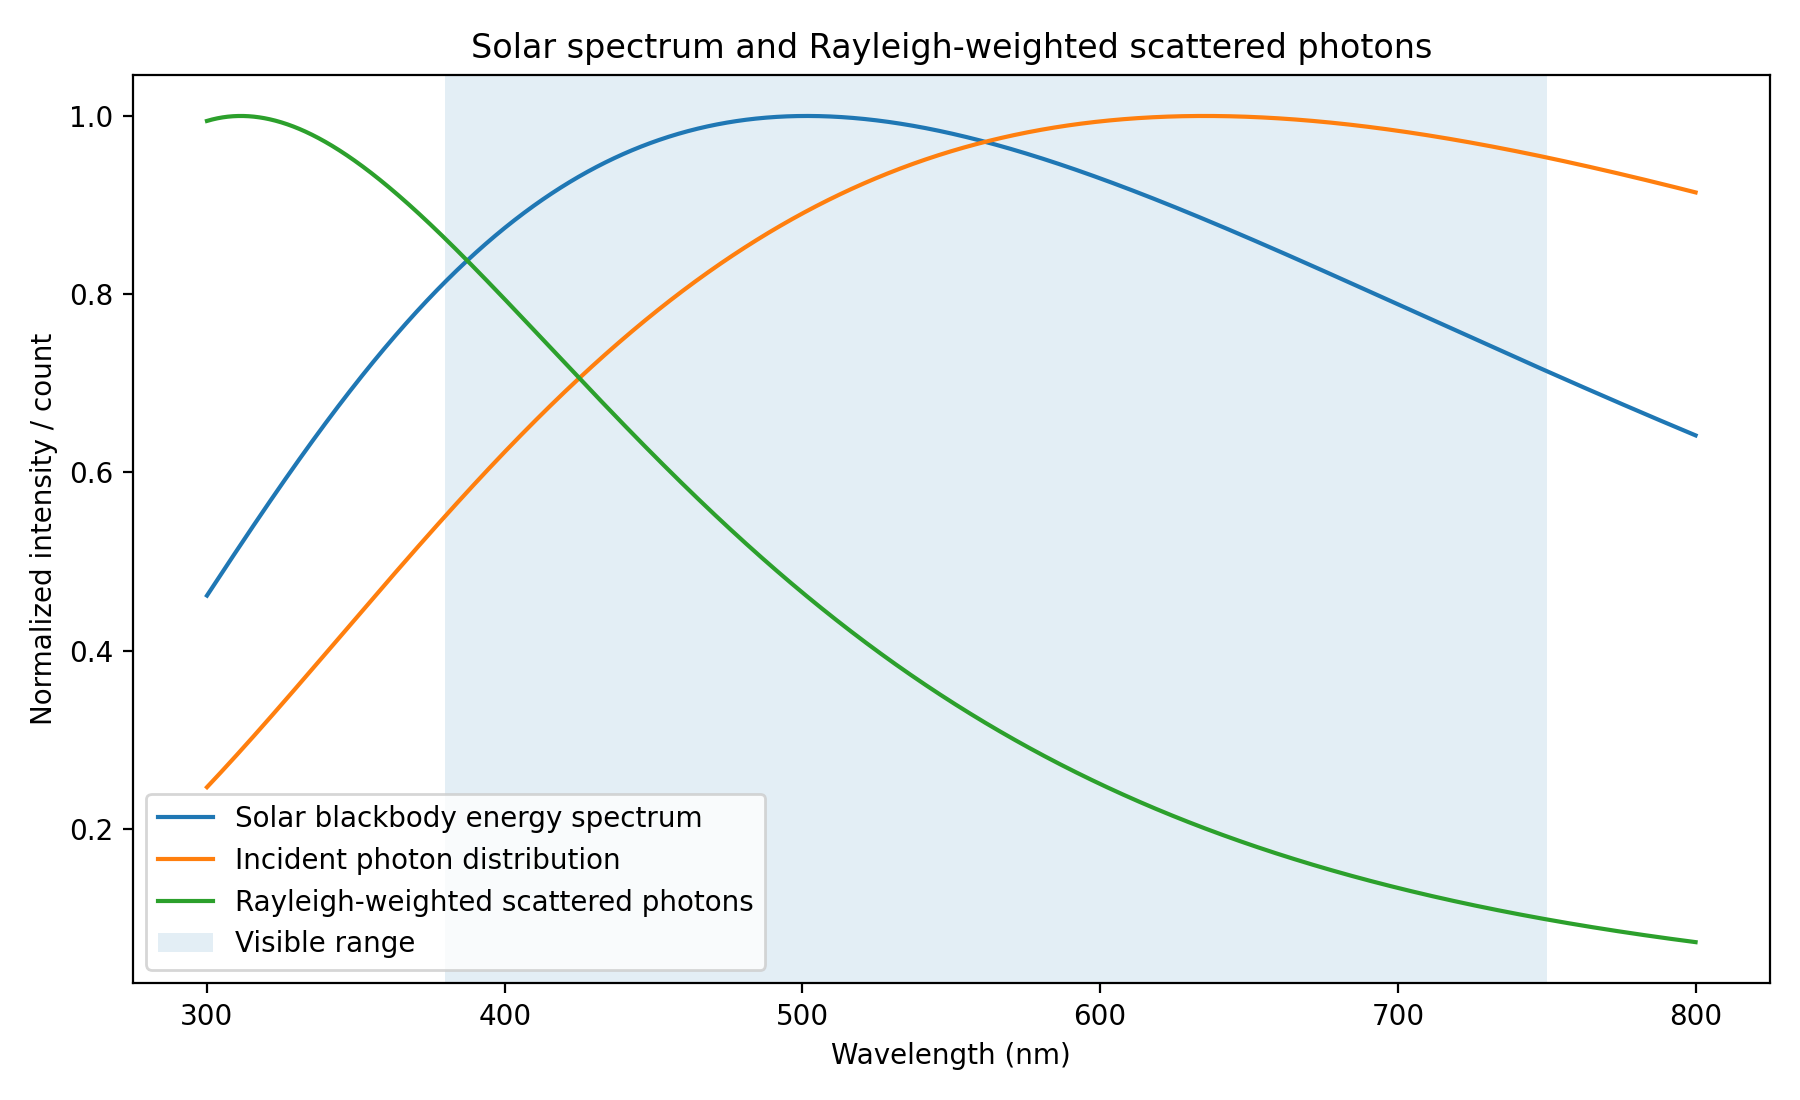
\includegraphics[width=0.92\textwidth]{rayleigh_scattering_solar_spectrum_figure.png}
\caption{Normalized comparison between a solar blackbody energy spectrum, the
corresponding incident photon distribution, and the Rayleigh-weighted
distribution of scattered photons, all plotted as functions of wavelength. The
scattered-photon curve is proportional to \(\lambda^{-4}\) times the incident
photon distribution. The visible range is shaded for reference.}
\label{fig:solar_rayleigh}
\end{figure}

\section{Discussion: Structural Clarification and Conceptual Seeing}

This paper is not pedagogical by reducing the phenomenon to a simple image or
an easily memorized rule. Rather, it is clarifying by refusing to stop at the
rule. Its aim is to expose the chain of dependencies that connects a common
optical phenomenon to the geometrical structure of electromagnetic theory.

The common explanation of the blue sky is correct but compressed. It says that
blue light is scattered more strongly, but it often hides the physical chain
behind this statement. A full explanation requires several layers of theory.

First, light is an electromagnetic field. Second, a small molecule in the
field is polarized and becomes an induced dipole. Third, the oscillating dipole
radiates because accelerated charges radiate according to Maxwell's equations.
Fourth, the far-zone radiation field is proportional to the second derivative
of the dipole moment. Fifth, electromagnetic intensity is not linear in the
field but quadratic, because it is part of the stress-energy structure of the
field. These facts together imply the fourth-power wavelength dependence of
Rayleigh scattering.

This is what is meant here by conceptual seeing. The point is not merely to
know that \(I_{\mathrm{sc}}\propto\lambda^{-4}\), but to see the formula as
an expression of a structure. In this respect the derivation is close in
spirit to Hanson's claim that seeing in science is theory-laden. The relevant
theoretical structure does not merely decorate an otherwise neutral
observation. It allows the phenomenon to be seen as what it is: not simply a
blue colour overhead, but a macroscopic appearance of dipole radiation and
electromagnetic stress-energy flow.

Spacetime algebra strengthens this point. The electromagnetic field is a
single bivector \(F\). Electric and magnetic fields are projections relative
to a chosen timelike direction \(u\). The molecule responds to \(F\cdot u\),
the electric field in its own rest frame. The frequency entering the response
is \(k\cdot u\), the projection of the incident null wave vector onto that
same timelike direction. The scattered radiation is an outgoing bivector
determined by the transverse dipole acceleration. The intensity is obtained
from the stress-energy map
\[
T_{F_{\mathrm{sc}}}(a)
=
-\frac{\varepsilon_0}{2}F_{\mathrm{sc}}aF_{\mathrm{sc}}.
\]
Thus Rayleigh scattering is not merely an optical formula, but a direct
consequence of the geometry and dynamics of the electromagnetic field.

This kind of explanation is not elementary, but it is clarifying. It is meant
for a reader who already has enough physics to recognize the ingredients, but
who wants to see why they belong together. In that sense, the question
``Why is the sky blue?'' becomes a test case for a deeper conception of
understanding in physics: not the ability to quote a formula, but the ability
to see how the formula follows from the structure of the theory.

\section{Conclusion}

The blue colour of the sky is a visible consequence of Rayleigh scattering.
But Rayleigh scattering itself is not a primitive fact. It follows from the
interaction between an incident electromagnetic field and small polarizable
molecules. In the Rayleigh regime, each molecule behaves as a driven electric
dipole; in quantum language, this is the classical limit of an off-resonant
elastic process mediated by virtual molecular excitations. The far radiation
field of this dipole is proportional to \(\omega^2\), while the observed
intensity is quadratic in the field. The result is

\begin{equation}
I_{\mathrm{sc}}
\propto
\omega^4
\propto
\frac{1}{\lambda^4}.
\end{equation}

In spacetime algebra this derivation takes a compact geometric form:

\begin{equation}
F_{\mathrm{in}}
\rightarrow
F_{\mathrm{in}}\cdot u
\rightarrow
p
\rightarrow
\ddot{p}
\rightarrow
F_{\mathrm{sc}}
\rightarrow
T_{F_{\mathrm{sc}}}(u)\cdot n.
\end{equation}

The sky is blue because the electromagnetic field, when projected into the
rest frames of atmospheric molecules, drives small dipoles whose radiation
field and stress-energy structure favour shorter wavelengths. The everyday
appearance of the sky is therefore a macroscopic trace of the geometric
structure of Maxwell theory.

\begin{thebibliography}{10}

\bibitem{Rayleigh}
Lord Rayleigh,
``On the light from the sky, its polarization and colour,''
\textit{Philosophical Magazine},
vol. 41, pp. 107--120, 1871.

\bibitem{Jackson}
J. D. Jackson,
\textit{Classical Electrodynamics},
3rd ed.,
Wiley, 1999.

\bibitem{Griffiths}
D. J. Griffiths,
\textit{Introduction to Electrodynamics},
4th ed.,
Pearson, 2013.

\bibitem{BohrenHuffman}
C. F. Bohren and D. R. Huffman,
\textit{Absorption and Scattering of Light by Small Particles},
Wiley, 1983.

\bibitem{BornWolf}
M. Born and E. Wolf,
\textit{Principles of Optics},
7th ed.,
Cambridge University Press, 1999.

\bibitem{Hestenes}
D. Hestenes,
\textit{Space-Time Algebra},
Gordon and Breach, 1966.

\bibitem{DoranLasenby}
C. Doran and A. Lasenby,
\textit{Geometric Algebra for Physicists},
Cambridge University Press, 2003.

\bibitem{Baylis}
W. E. Baylis,
\textit{Electrodynamics: A Modern Geometric Approach},
Birkh\"auser, 1999.

\bibitem{Hanson}
N. R. Hanson,
\textit{Patterns of Discovery: An Inquiry into the Conceptual Foundations of Science},
Cambridge University Press, 1958.

\bibitem{Kuhn}
T. S. Kuhn,
\textit{The Structure of Scientific Revolutions},
University of Chicago Press, 1962.

\end{thebibliography}

\end{document}
